\documentclass{beamer}
% \usetheme[framenumber,technologie]{AP}

\usepackage[dutch]{babel}

\title[]{Embedded Development}
\subtitle{met het Microsemi SmartFusion Platform}
\author{}
\institute{Jeroen Doggen\\ jeroen.doggen@artesis.be \\Artesis Hogeschool Antwerpen}
\date{Versie: \today}

\AtBeginSubsection[]
{
  \begin{frame}<beamer>
    \frametitle{Overzicht}
    \tableofcontents[currentsection,currentsubsection]
  \end{frame}
}

\AtBeginSection[]
{
  \begin{frame}<beamer>
    \frametitle{Overzicht}
    \tableofcontents[currentsection,currentsubsection]
  \end{frame}
}

\begin{document}

% Titlepage 
\maketitle

% Outline Page
\section*{Overzicht}
\begin{frame}
\frametitle{Overzicht}
\tableofcontents
\end{frame}


%=============================================================================================================================%
\section{Inleiding}
%=============================================================================================================================%

\begin{frame} 
\frametitle{SmartFusion Evaluation Board}

% \begin{itemize}
%  \item test
% \end{itemize}
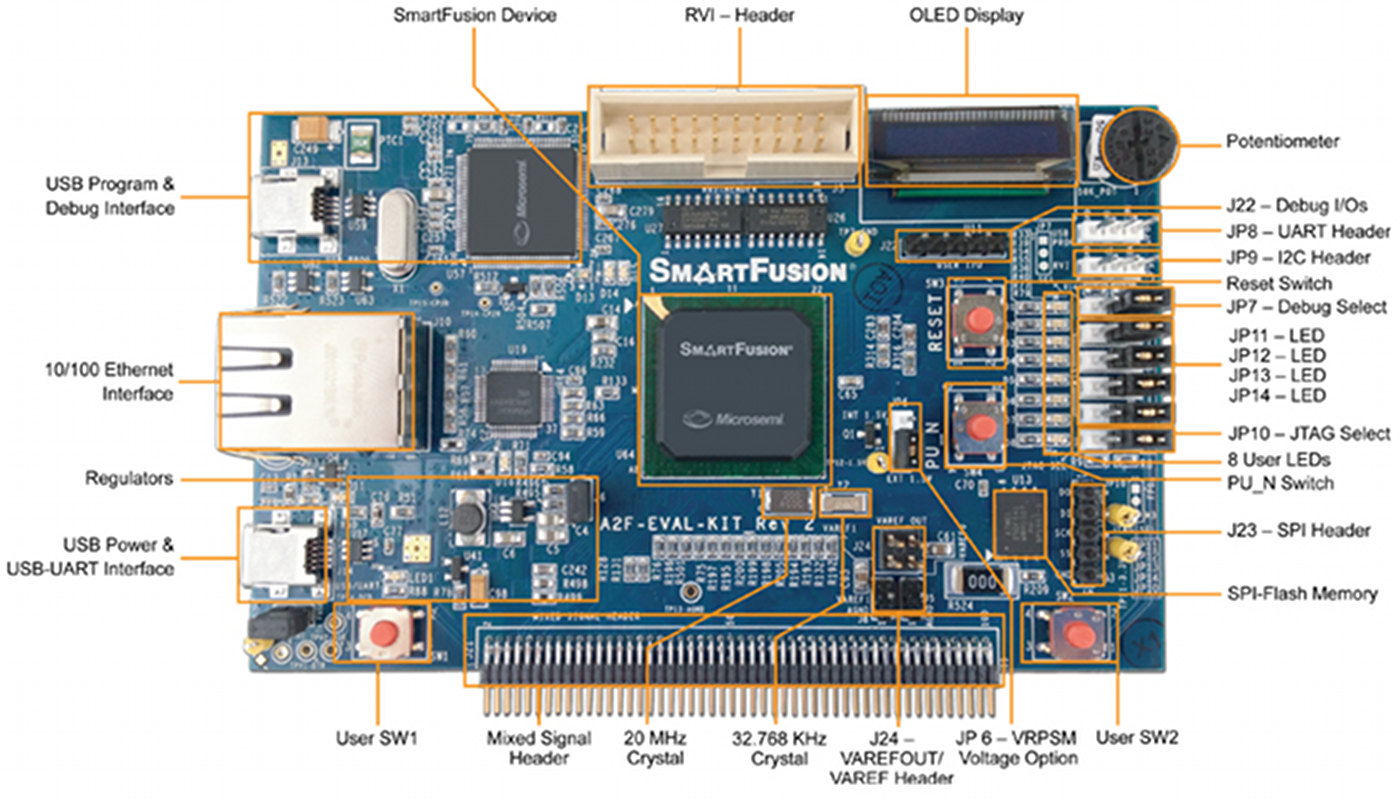
\includegraphics[width=1\textwidth]{./images/SmartFusion.jpeg}

Intro film: %\url{http://www.actel.com/FPGA/SmartFusion/video/intro_hires.html}
\url{http://www.youtube.com/watch?v=KY9eKF0llms} %(dezelfde film)
\end{frame}


%=============================================================================================================================%
\subsection{Traditioneel Embedded Design}
%=============================================================================================================================%

\begin{frame} 
\frametitle{Ontwikkeling van een ``Product''}
\begin{itemize}[<+->]
 \item Tijdens een volledig design worden verschillende stappen doorlopen
 \item In grote projecten zal iedere stap van een design de verantwoordelijkheid van een team zijn.
 \item Vereenvoudigde voorstelling:
 \begin{itemize}
    \item Vaststellen van een probleem of vraag naar een toepassing
    \item Analyse van het probleem
    \item Ontwerp van een conceptuele oplossing
    \item Ontwerp van de hardware \footnote{Dit valt volledig binnen ons vakgebied.}
    \item Ontwerp van de software \footnotemark[1]
    \item Mechanisch/fysiek ontwerp
 \end{itemize}
\end{itemize}
\end{frame}

%=============================================================================================================================%

\begin{frame} 
\frametitle{Voorbereidende stappen}

\begin{itemize}[<+->]
\item Vaststellen van een probleem of vraag naar een toepassing
  \begin{itemize}
  \item Uitvoeren van een marktonderzoek
  \item Financi\"ele analyse
  \end{itemize}
\item Analyse van het probleem
\begin{itemize}
 \item Wat zijn de noden van de gebruiker
 \item Waarom is er een vraag naar een oplossing
 \item Wie zijn de potenti\"ele klanten
\end{itemize}
\item Ontwerp van een conceptuele oplossing
\begin{itemize}
 \item Uitwerken van de oplossing aan de hand van een mock-up
 \item Ontwerp van een niet-functioneel prototype
 \item Uitvoeren gebruikerstests
\end{itemize}
\end{itemize}
\end{frame}

%=============================================================================================================================%

\begin{frame} 
\frametitle{Embedded Hardware Design}

\begin{itemize}[<+->]
\item Ontwerp van een hardware prototype op een breadboard (microcontroller schakeling)
\item Ontwerp van een hardware prototype op een gatenprint
\item Ontwerp van printed-circuit board (PCB)
\item Productie van PCB (etsen/frezen)
\item Bestukken en testen van PCB
\end{itemize}

% ++ TESTING

\end{frame}

%=============================================================================================================================%

\begin{frame} 
\frametitle{Embedded Processing Unit}
\begin{itemize}[<+->]
  \item De hardware wordt uitgerust met een microcontroller
  \item Dit is een processor met extra mogelijkheden naar I/O interfacing toe
    \begin{itemize}
    \item Analoog Digitaal Converters (ADC)
    \item Seri\"ele communicatie: UART, SPI, I2C
    \item General Purpose Input Output pinnen (GPIO)
    \end{itemize}
  \item Er zal software geschreven worden die wordt uitgevoerd door deze processor (meestal C/C++)
  \item Voordeel: flexibiliteit, aanpasbaarheid, vlotte communicatie tussen devices 
\end{itemize}
\end{frame}

%=============================================================================================================================%

\begin{frame} 
\frametitle{Embedded Software Design}
\begin{itemize}[<+->]
  \item Ontwerp van een software architectuur: bouwstenen, lagen, functionele blokken,...
  \item Schrijven/gebruiken van bibliotheken voor I/O interfacing
  \item Ontwerp van een ``main'' applicatie: State machine, interrupt based, real-time operating system (RTOS),...
  \item Bij normaal uitvoeren van een embedded toepassing: beperkt zicht op wat software aan het doen is
  \item On-chip debuggen van de toepassing: toepassing stap-per-stap uitvoeren om fouten op te sporen (plaatsen breakpoints, geheugeninhoud bekijken \& aanpassen).
\end{itemize}
\end{frame}

%=============================================================================================================================%
\subsection{Hardware / Software Co-design}
%=============================================================================================================================%

\begin{frame} 
\frametitle{Programmeerbare Logica}
\begin{columns}[c] 
\column{.7\textwidth} 
  \begin{itemize}[<+->]
    \item Field Programmable Gate Array (FPGA)
    \item Volledig herprogrammeerbaar alternatief voor een ASIC
    \item Een FPGA wordt normaal gebruikt om custom gedrag in een chip te implementeren. (ALU, counters, state machines,...)
    \item Voordeel: flexibiliteit \& aanpasbaarheid: rekenkracht en I/O mogelijkheden
  \end{itemize}
\column{.35\textwidth} 
  \begin{figure}[h]
  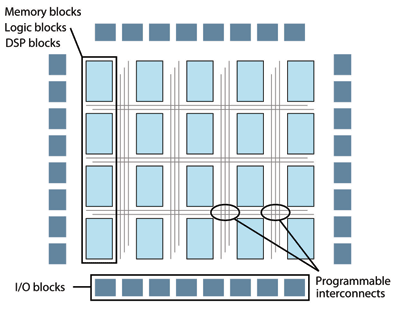
\includegraphics[width=0.99\textwidth]{images/fpga.png}
  \end{figure}
\end{columns}
\end{frame}

%=============================================================================================================================%

\begin{frame} 
\frametitle{Programmeerbare Logica}
\begin{columns}[c] 
\column{.5\textwidth} 
  \begin{itemize}[<+->]
    \item Bij FPGA programmeren worden o.a. de volgende twee stappen uitgevoerd:
    \begin{enumerate}
     \item De logische opbouw van de schakeling ontwerpen.
     \item De manier waarop de schakeling met de buitenwereld is verbonden vastleggen. (mapping van fysieke naar logische pinnen)
     \end{enumerate}
   \end{itemize} 
\column{.55\textwidth} 
  \begin{figure}[h]
  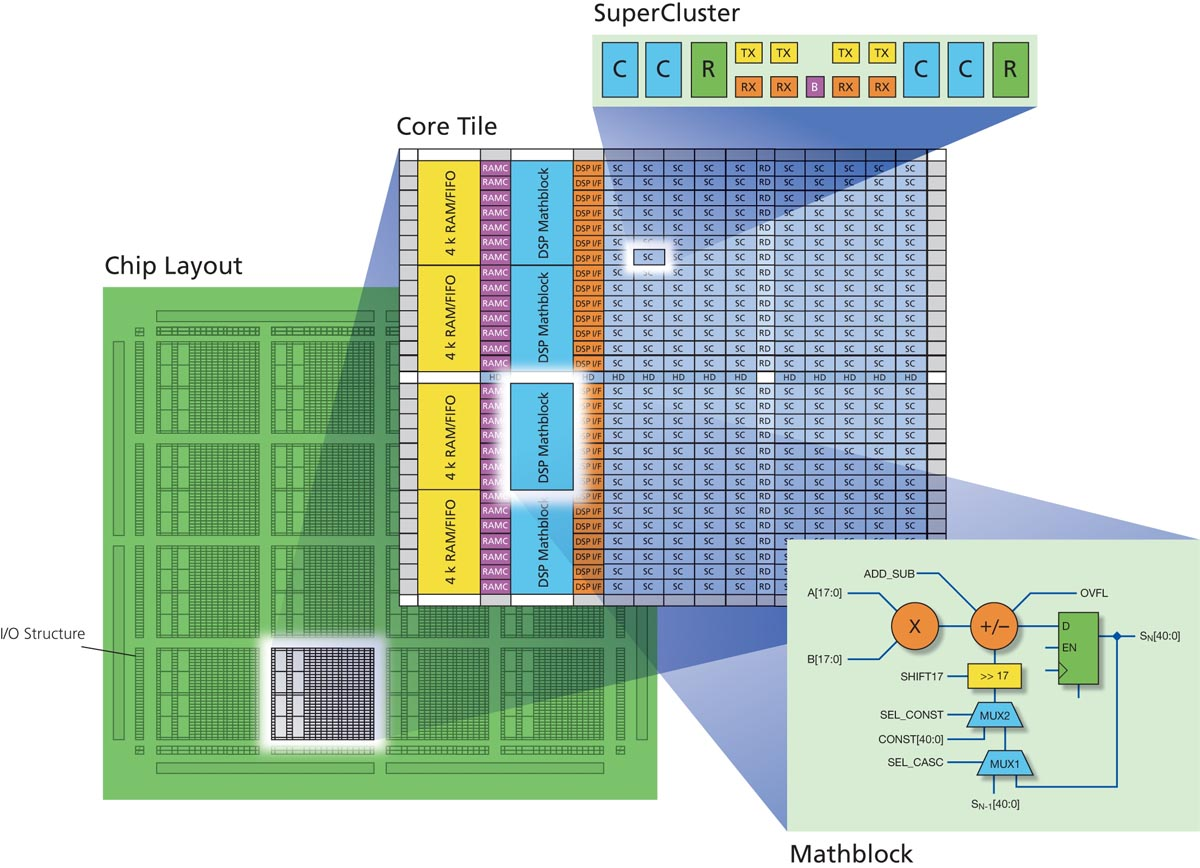
\includegraphics[width=0.99\textwidth]{images/fpga2.jpg}
  \end{figure}
\end{columns}
\end{frame}

%=============================================================================================================================%

\begin{frame} 
\frametitle{Samenvoegen FPGA \& Microcontroller}
 \begin{itemize}[<+->]
   \item Zowel een FPGA als een microcontroller heeft zijn voordelen:
    \begin{itemize}
      \item Microcontroller: development tijd, aanpasbaarheid, vlotte communicatie tussen devices 
      \item FGPA: rekenkracht en I/O mogelijkheden
      \end{itemize}
    \item Door de twee te combineren kunnen we de voordelen van de twee types combineren.
      \begin{itemize}
       \item We kunnen toepassingen ontwikkelen in C en deze laten communiceren met zelf ontworpen hardware.
       \item Daarnaast kan de toepassing eenvoudig via de UART met een PC verbonden worden.
       \item Dit alles zonder de echte hardware te moeten aanpassen. (``zonder soldeerbout'')
      \end{itemize}
   \end{itemize} 
\end{frame}


%=============================================================================================================================%

\begin{frame} 
\frametitle{Microsemi SmartFusion}
  \begin{figure}[h]
  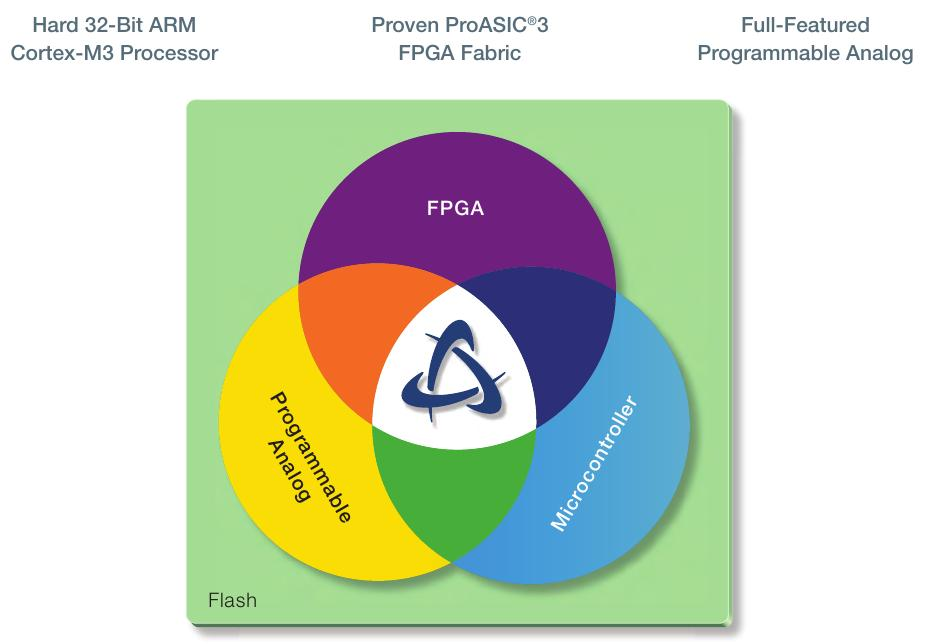
\includegraphics[width=0.9\textwidth]{images/fusiondiagram.jpeg}
  \end{figure}
\end{frame}

%=============================================================================================================================%

\begin{frame} 
\frametitle{Microsemi SmartFusion}
  \begin{figure}[h]
  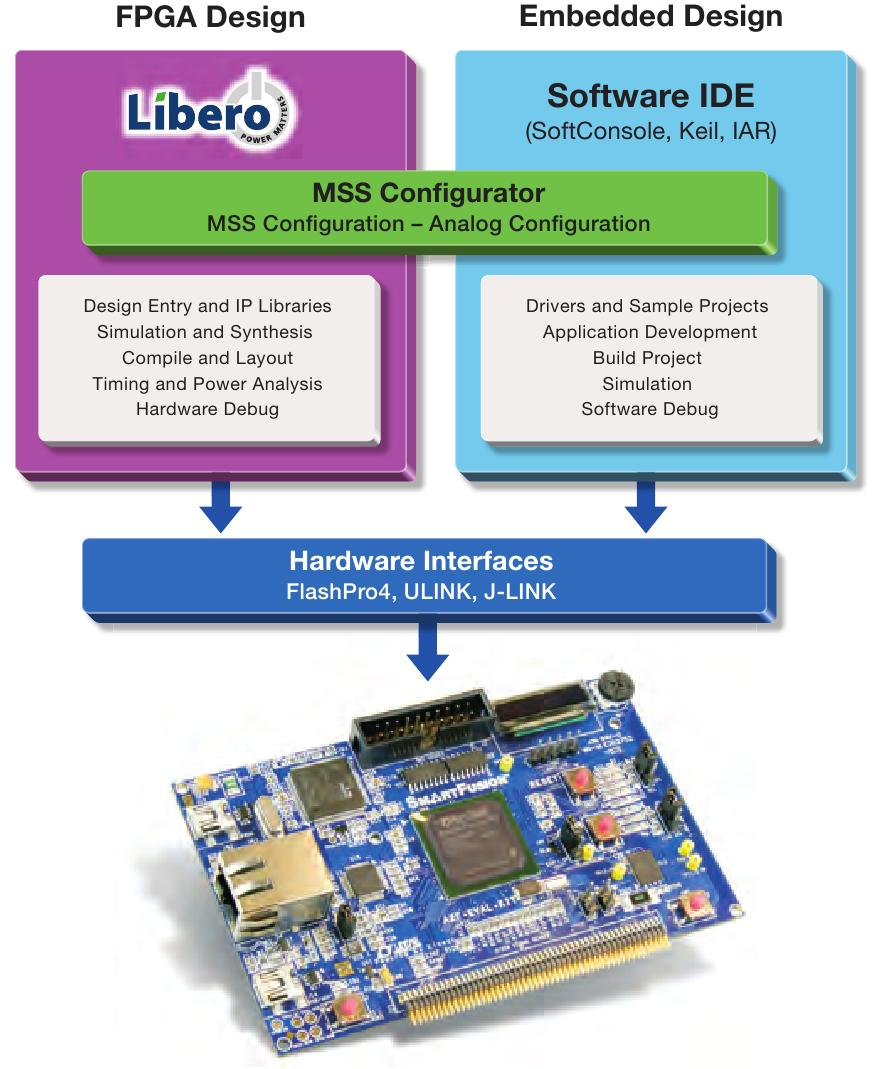
\includegraphics[width=0.53\textwidth]{images/designtools.jpeg}
  \end{figure}
\end{frame}

%=============================================================================================================================%

\begin{frame} 
\frametitle{Microsemi SmartFusion}
  \begin{figure}[h]
  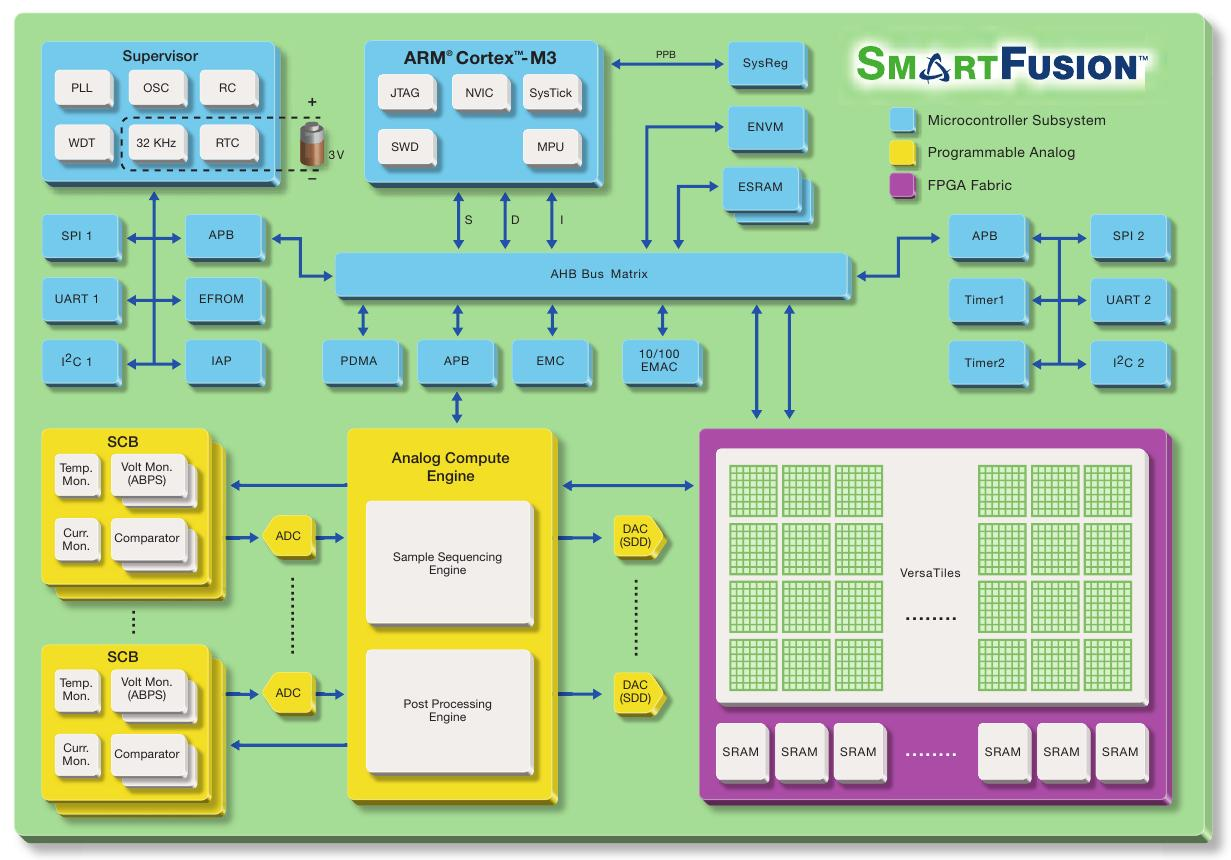
\includegraphics[width=0.92\textwidth]{images/fusionblockdiagram.jpeg}
  \end{figure}
\end{frame}

%=============================================================================================================================%

\begin{frame} 
\frametitle{Alternatieven: Zynq-7000 (Xilinx)}
  \begin{figure}[h]
  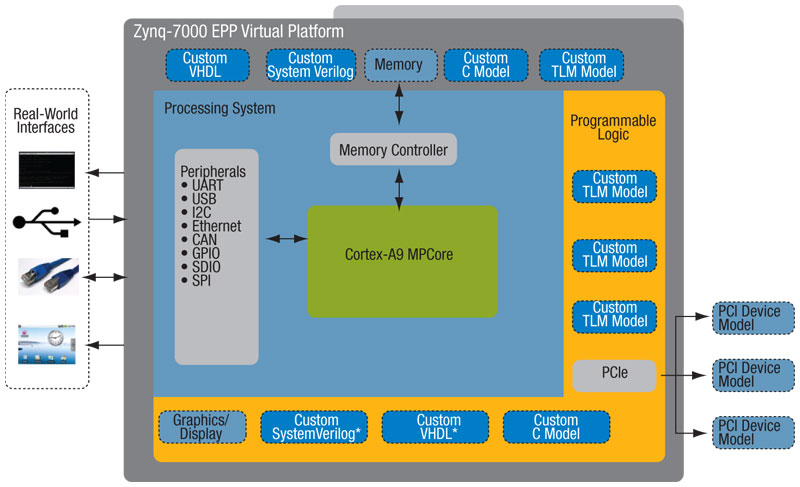
\includegraphics[width=0.95\textwidth]{images/zynq.jpg}
  \end{figure}
\end{frame}

%=============================================================================================================================%

\begin{frame} 
\frametitle{Alternatieven: Atom E6x5C Serie (Intel/Altera)}
  \begin{figure}[h]
  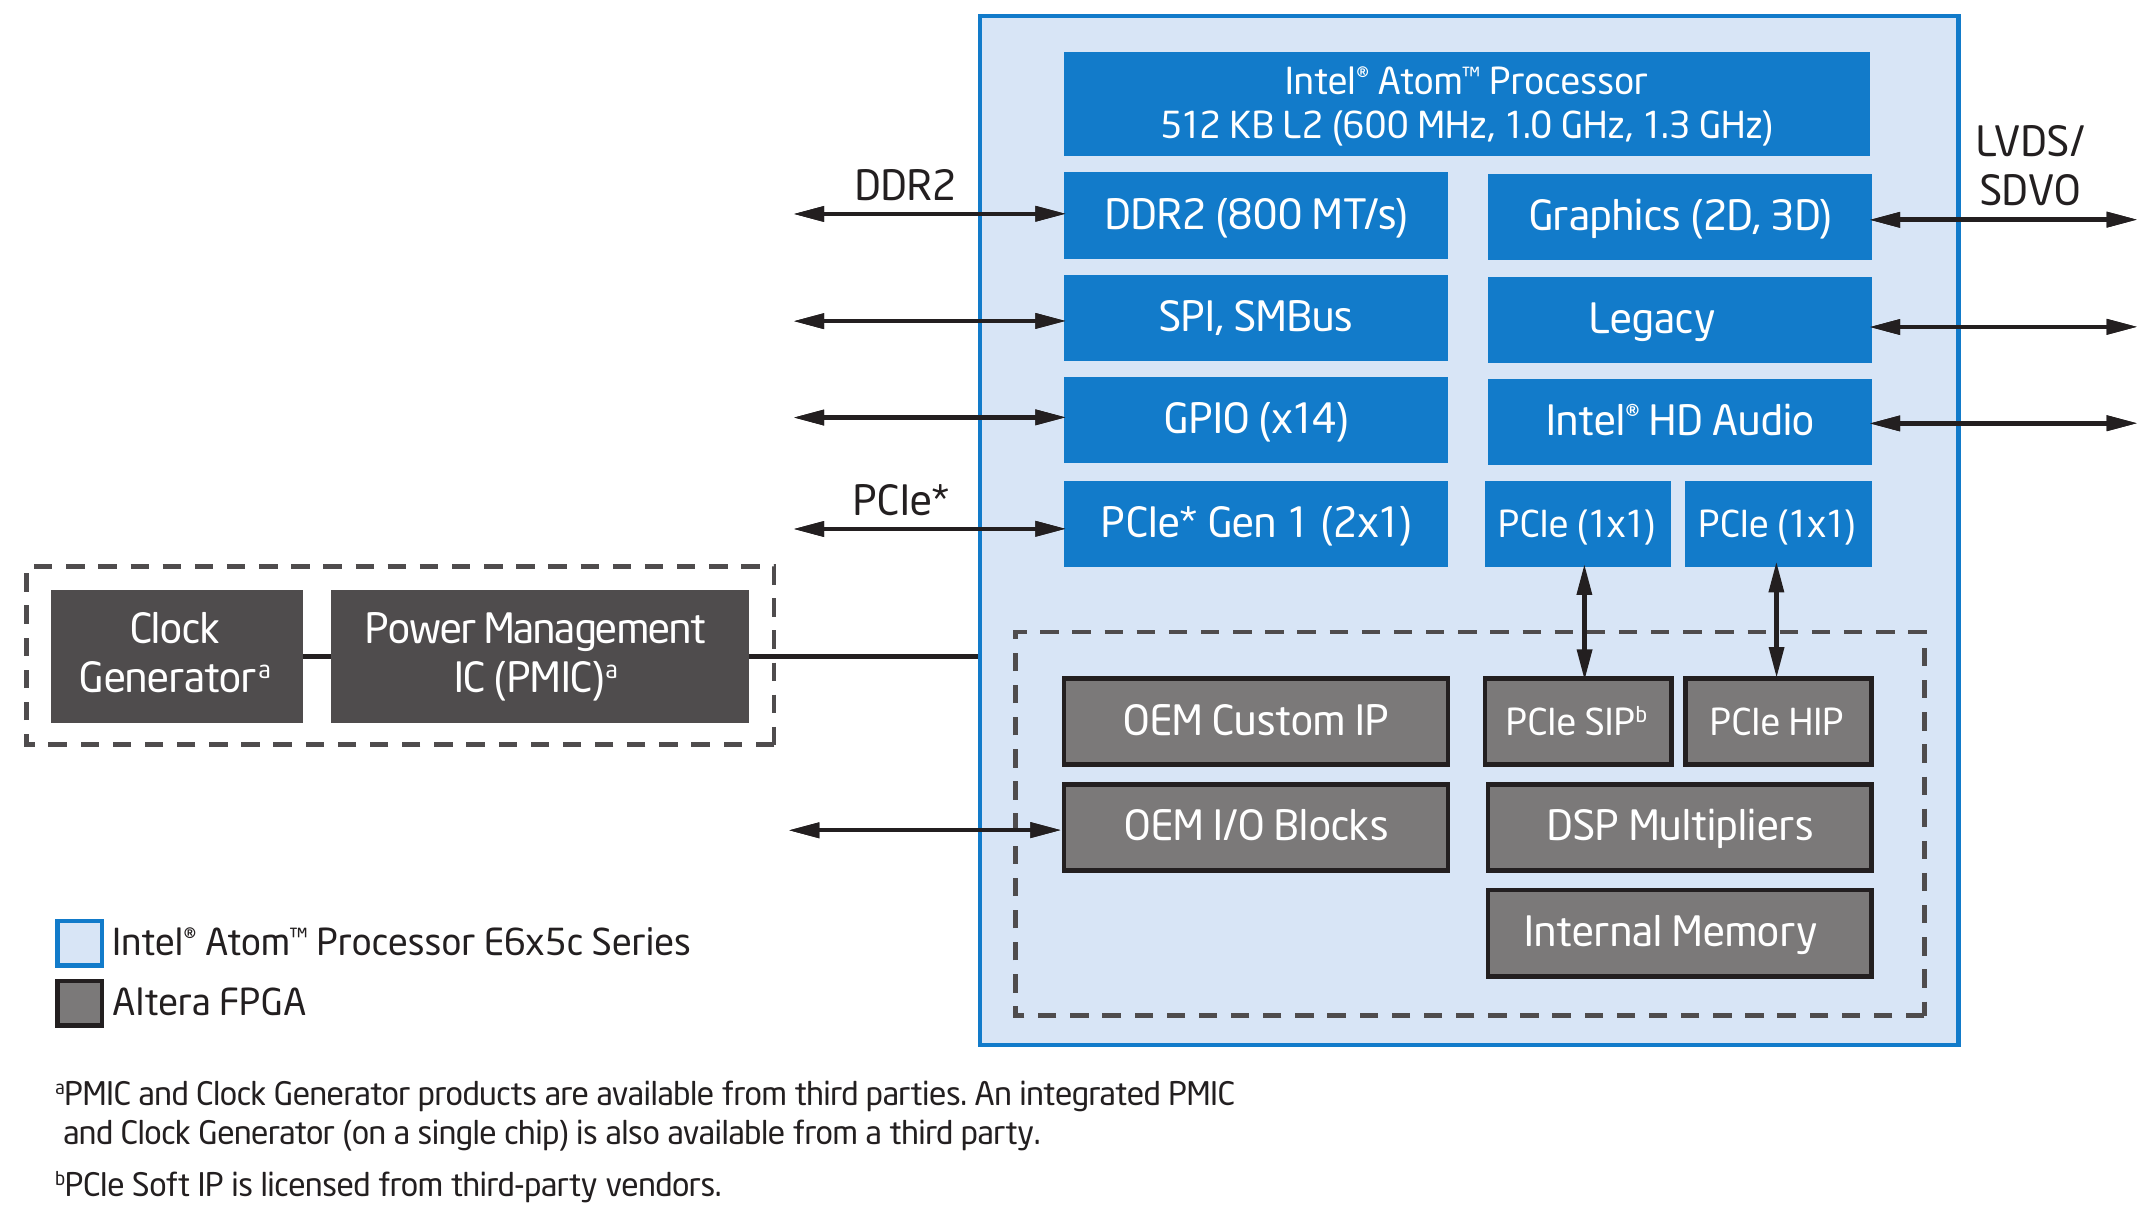
\includegraphics[width=0.95\textwidth]{images/atomFPGA.png}
  \end{figure}
\end{frame}

%=============================================================================================================================%
\section{Overzicht Design Flow}
%=============================================================================================================================%

% \begin{frame} 
% \frametitle{Placeholder}
%   \begin{itemize}[<+->]
%     \item placeholder
%   \end{itemize}
% \end{frame}

%=============================================================================================================================%
\subsection{Configuratie SoC}
%=============================================================================================================================%

\begin{frame} 
\frametitle{Configuratie SoC}
  \begin{itemize}
    \item Gebeurt m.b.v. ``Libero: MSS Configurator''
    \item Configureer de microcontroller
    \begin{itemize}
      \item Stel in welke I/O devices actief zijn
      \item Stel klokfrequentie van de microcontroller in
    \end{itemize}
    \item Plaats eventueel extra schakelingen in de FPGA
  \end{itemize}
\end{frame}

%=============================================================================================================================%
\subsection{Hardware ``Synthese''}
%=============================================================================================================================%

\begin{frame} 
\frametitle{Hardware ``Synthese''}
  \begin{itemize}[<+->]
    \item Gebeurt m.b.v. ``Synplify Pro''
    \item Doorloop de nodige stappen op de configuratie uit de vorige stap om te vormen tot een bestand dat kan geupload worden naar de SoC
    \item Deze stappen verlopen ons geval zo goed als automatisch: mits de juiste instellingen zijn gekozen
      \begin{itemize}
      \item Welke FPGA/SoC is in gebruik
      \item Zijn de licentie van de software tools correct ge\"installeerd
      \end{itemize}
  \end{itemize}
\end{frame}

%=============================================================================================================================%
\subsection{Programmeren SoC}
%=============================================================================================================================%

\begin{frame} 
\frametitle{Programmeren SoC}
  \begin{itemize}[<+->]
    \item Gebeurt m.b.v. ``Flashpro''
    \item Uploaden van het hardware design naar de SoC
    \item Indien je in de vorige stap het hardware designbestand opslaat kan je in volgende projecten/oefeningen waar dezelfde configuratie nodig is de voorgaande stappen overslaan.
  \end{itemize}
\end{frame}

%=============================================================================================================================%
\subsection{Software/Firmware Ontwikkeling}
%=============================================================================================================================%

\begin{frame} 
\frametitle{Software/Firmware Ontwikkeling}
  \begin{itemize}[<+->]
    \item Gebeurt m.b.v. ``Softconsole (een re-branded Eclipse IDE)''
\end{frame}

%=============================================================================================================================%
\subsection{Firmware Debugging}
%=============================================================================================================================%

\begin{frame} 
\frametitle{Placeholder}
  \begin{itemize}[<+->]
    \item Gebeurt m.b.v. ``GDB/OpenOCD''
  \end{itemize}
\end{frame}

%=============================================================================================================================%
\section{Voorbeeldtoepassingen}
%=============================================================================================================================%

\begin{frame} 
\frametitle{Placeholder}
  \begin{itemize}[<+->]
    \item placeholder
  \end{itemize}
\end{frame}

%=============================================================================================================================%
\end{document}
%=============================================================================================================================%